\documentclass[10pt,a4paper]{article}
\usepackage[utf8]{inputenc}
\usepackage[francais]{babel}
\usepackage[T1]{fontenc}
\usepackage{hyperref}
\usepackage{eurosym}
\usepackage{ amssymb }
\usepackage{graphics}
\usepackage{pdfpages}

\begin{document}

\begin{titlepage}
    \begin{center}
        \textbf{\textsc{UNIVERSIT\'E LIBRE DE BRUXELLES}}\\
        \vfill{}\vfill{}
        \begin{center}{\Huge Rapport : Villo !}\end{center}{\Huge \par}
        \begin{center}{\large Romain \textsc{Fontaine}, Nikita \textsc{Marchant}}\end{center}{\Huge \par}
        \vfill{}\vfill{} \vfill{}
        \begin{flushleft}{\large \textbf{INFO-H-303 Base de données}}\hfill{Esteban Zimányi, Michaël Waumans}\end{flushleft}{\large\par}
        \vfill{}\vfill{}\enlargethispage{3cm}
        \textbf{Année académique 2015--2016}
    \end{center}
\end{titlepage}

\setlength{\parindent}{1.5em}
\setlength{\parskip}{1em}
\linespread{1.1}


% \tableofcontents

% \pagebreak


\section{Diagramme entité association}
\subsection{Diagramme}

Le diagramme se trouve en annexe, page \pageref{diagram}.

\begin{figure}[Hbt]
    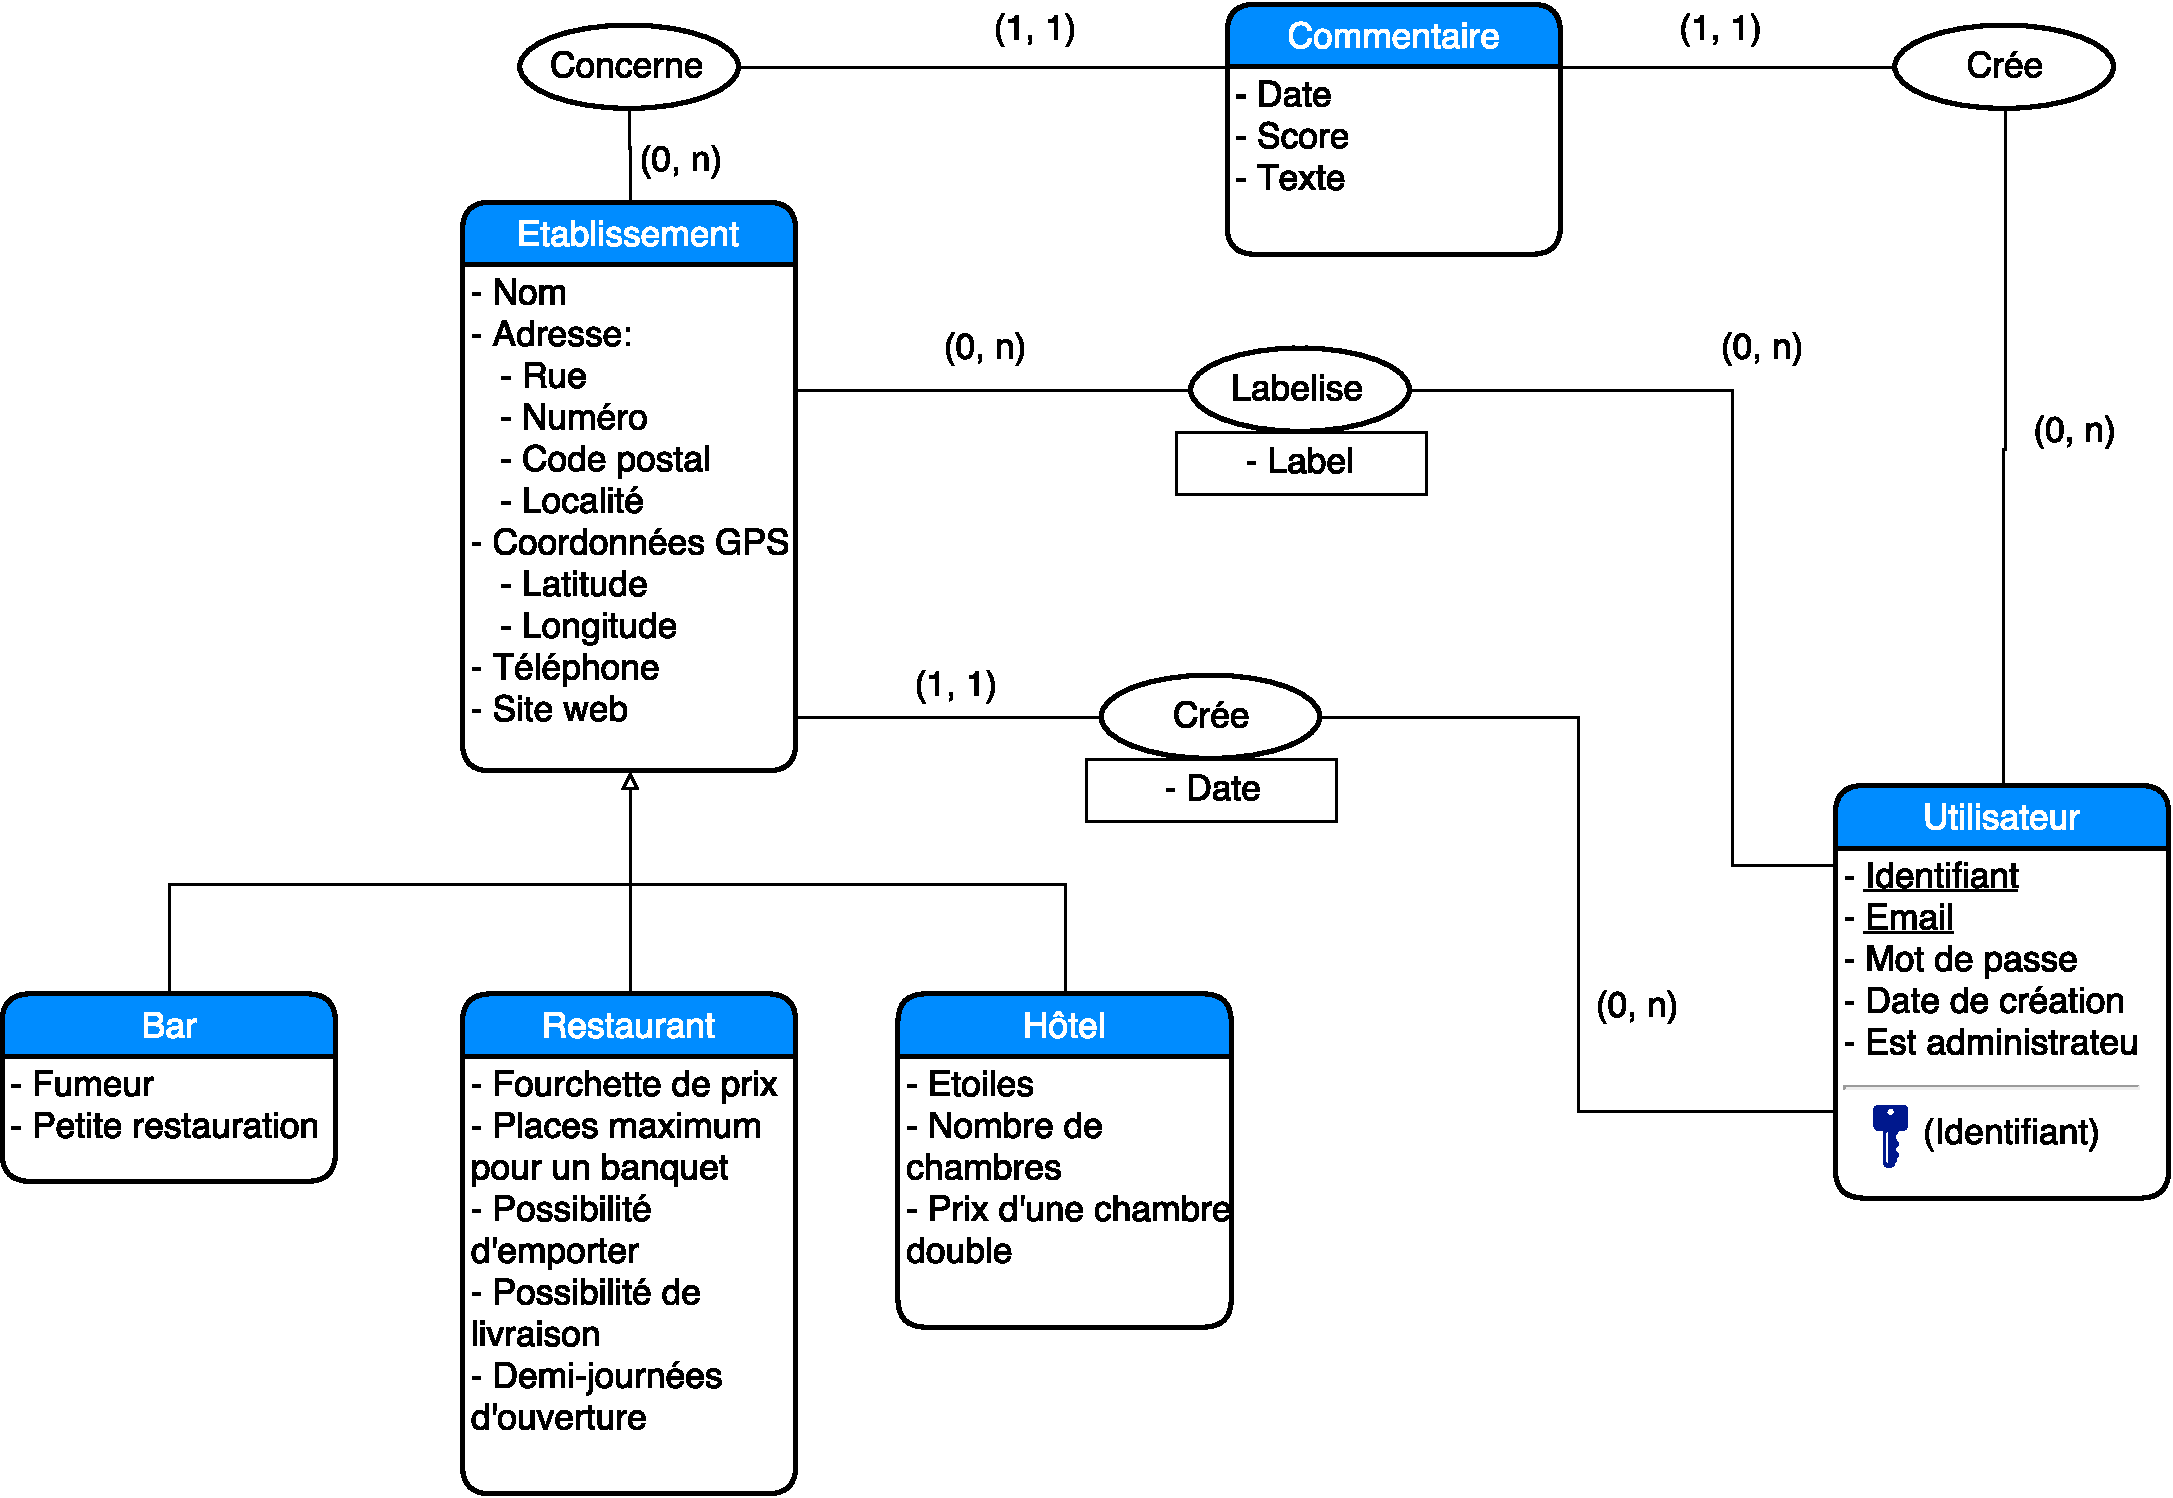
\includegraphics[angle=90, scale=0.6]{EA.pdf}
    \caption{Diagramme Entité-Association}
    \label{diagram}
\end{figure}
\subsection{Contraintes}
Les contraintes sont les suivantes :
\begin{itemize}
  \item ...
\end{itemize}



\section{Modèle relationnel}
\subsection{Modèle}


\begin{description}

\end{description}

\subsection{Contraintes}

Les contraintes sont les suivantes :
\begin{itemize}
  \item ...
\end{itemize}

\section{Hypothèses}

...

\section{Justification}

Afin d'éviter la redondance et de garantir la cohérence du modèle, nous avons choisis de :
\begin{itemize}
  \item ...
\end{itemize}
En effet, ...



\end{document}

